\chapter{Problem analysis}\label{ch:ProblemAnalysis}
In order to gain a deeper understanding of the problem domain, a problem analysis is conducted to scrutinise the underlying problems. In this chapter we define what \textit{Home Automation} is and which technologies are required, in order to get a deeper understanding of which features PHAL should support.

\section{Home Automation}
There are several different terms associated with computer controlled houses, such as 'Smart Home', 'Smart House' and 'Home Automation'. According to the book Smart Home Systems Chapter 1, Section 3, such a system is described as follows:
\begin{quote}
\textit{An automated home typically allows the control of room  luminosity,  opening  and  closing  of  shutters,  heating and  air  conditioning,  or multimedia systems. Home  applications  main  objective  is  the comfort  and simplification  of  the  daily  life  of residents,  and  home  support  of  elderly or  convalescents.}
\end{quote}
Following this definition, the more rigid definition, according to the EP1260886A2 patent (\cite{EP1206886A2}) is:
\begin{quote}
\textit{Home automation system \textit{(31}) comprising an array of functional devices \textit{(37)}, a plurality of input devices \textit{(38)} associated with the array of functional devices and a control unit \textit{(49)}, interconnected via radio link and constituting a home automation system \textit{(32)} \dots}
\end{quote}
Given these two definitions, anything electronic can, in theory, be included within a home automation system. This means that there are endless possible combinations as to what is connected to the systems. Due to this, PHAL will be focused on a narrow sub-part of home automation, due to the limited time and hardware at our disposal. This sub-part will be described later during this chapter, where only a small number of devices will be supported by PHAL.

\section{Platforms for home automation}
In the following section we will investigate the different hardware platforms suitable for creating a home automation system. We will take a more detailed look into the chosen platform and the current language thereto in order to gather information and find limitations in order to discover what can be improved in PHAL. 

\subsection{Choosing a platform}\label{PlatformsForHomeAutomation}
There are many different hardware platforms to choose from when creating a home automation system. Most of the available platforms are very similar in terms of hardware layout. However, they may differ in complexity and price. As seen on Table~\ref{tab:Platforms}, the major difference between the platforms is the price and the power voltage needed to operate the board.
\begin{table}[H]
\begin{center}
\begin{tabular}{|l|c|c|c|c|c|c|}
    \hline
    Name                                & Price     & Pins       & Output     & Memory      \\
                                        &           &            & power      &             \\\hline
    Arduino Uno R3 \cite{ArduinoUnoR3}  & 140 DKK   & 14         & 16 MHz     & 32 KB       \\\hline
    Raspberry Pi 3                      &           &            &            &             \\
    model B \cite{RaspberryPi3ModelB}   & 299 DKK   & 40         & 1.2 GHz    & 1 GB        \\\hline
    Intel Galileo \cite{IntelGalileo}   & 520 DKK   & 14         & 400MHz     & 256 MB      \\\hline
        Micro:bit \cite{MicroBit}           & 160 DKK   & 19         & 16MHz      & 256KB   \\\hline
\end{tabular}
\caption{The table shows the four different platforms and some of their pros and cons.}
\label{tab:Platforms}
\end{center}
\end{table}
\noindent
The price of a platform is essential in the decision making process when a hobbyist has to decide which platform to buy. If a given platform has similar specifications as other platforms, then the price is most likely going to be the deciding factor in which platform the hobbyist chooses to buy. 
\\
One of the things that limits the home automation systems which can be implemented using a given platform, is the native amount of pins available to connect input and output devices. It is therefore also important to consider this when choosing a platform.
\\
When creating a home automation system, the amount of calculations made by the control unit will presumably be relatively small, since it would only evaluate the input given to it in order to make a decision. Since a home automation system is not a time sensitive system the clock speed of the platform would not be significant when choosing a platform.
\\
When the platform receives information from its sensors and other input devices, the previous readings will typically not be stored in memory for long periods of time. Hence the memory available on the platform will not be significant when choosing a platform. 
\\\\
Based on the arguments listed above, the Arduino Uno platform has been chosen based primarily on its low price, which makes it an optimal match for hobbyists. Though the Arduino platform has a higher price per pin than the Raspberry Pi 3 model B, the Arduino can be extended with more general purpose input/output extension boards, providing a lower price per pin than the Raspberry Pi 3 model B.

\subsection{The Arduino platform}
Arduino is an open-source electronics platform, where the purpose of the platform is to make it easy to use hardware and software for educational purposes. 
The hardware of an Arduino is a circuit board which can read inputs from all sorts of different sensors such as ultrasound, light sensors or a temperature sensors connected to the female pins, which can be seen on Figure~\ref{fig:ArduinoUnoR3}. 
These can then be used in a program written for the Arduino, which in turn can produce different outputs. The output can, for example, be the ability to turn a light bulb on or off based on the input from the sensors. The instructions for Arduino are written in the Arduino Programming Language (APL) \cite{ArduinoLanguage}, which is based on the programming  languages C and C++. As a result of this, when the code is compiled it undergoes some changes, where the function calls are automatically generated in an intermediate language, afterwards the code is compiled with a C/C++ compiler called avr-g++ \cite{ArduinoLanguage}.
\begin{figure}[H]
\centering
  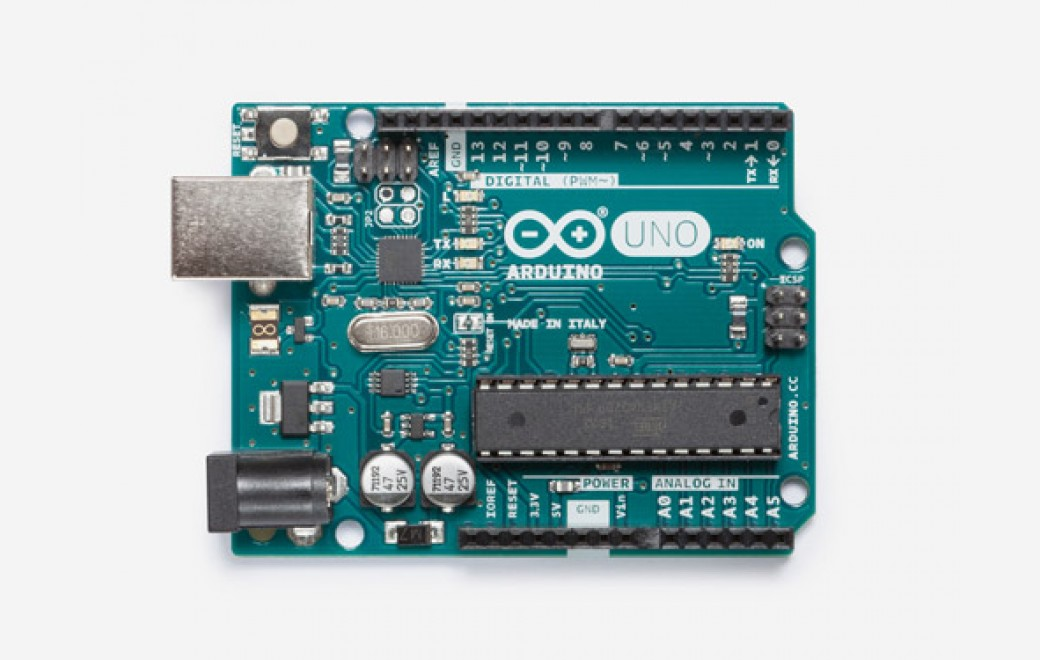
\includegraphics[width=\textwidth]{figures/Analysis/ArduinoUnoR3.jpg}
  \caption{This figure shows the Arduino Uno R3 board \cite{ArduinoUnoR3}.}
  \label{fig:ArduinoUnoR3}
\end{figure}
%\subsection{The use of Arduino}
\noindent
Arduino is designed to be easily accessible to all users, both experienced and inexperienced. The Arduino webside provides tutorials for beginners to learn how to program and use the language and platform. Furthermore, they have a dedicated community that is creating projects and sharing their experiences. The Arduino is inexpensive and readily available and would therefore be ideal for home automation projects due to its easy obtainability. Likewise, components for the Arduino are easy to obtain and are well documented on the internet which makes it ideal for the general hobbyist.

\section{Targeted users}\label{ProblemA:Users}
The intention with PHAL is to focus on the users with a limited amount of programming experience. Due to this, the language has to be intuitive and easy to understand and write. As mentioned in Subsection~\ref{ProblemA:ArduinoLanguage}, the Arduino is programmed in APL which is a c/c++ based language. APL inherits a lot of functionality from those languages, which makes it a powerful language, but not necessarily easily understandable.
\\\\
The focus of the PHAL language is to increase the level of abstraction for the user to create a much more simplistic and intuitive syntax, reducing the amount of programming knowledge needed to extract the full potential of the language when compared to APL. Because of the aim to reduce overall need of programming knowledge, the targeted users of our language are primarily hobbyists with no to little prior programming experience but some experience with electric circuits. 

\section{Technologies in a home}
In order to gain a deeper understanding of which technologies PHAL needs to support, an analysis of the technologies commonly used in a home automation system is conducted. 

\subsubsection{Lights}
The lights can be considered a basic element of any household. A light can be controlled in many different ways, such as by a button, light dimmer, through sensors or by timers. Given how essential lights are to a regular home, it is essential that the PHAL language needs the ability to control lights. This means PHAL should facilitate ease of using the lights through home automation \cite{BenefitsAndRisksOfSmartHomeTechnologies}.

\subsubsection{Heating systems and temperature sensors}
Roughly every home has some sort of climate control, such as radiators or heat pumps. An obvious use for a home automation system is as such to both monitor and control these aspects of the home \cite{BenefitsAndRisksOfSmartHomeTechnologies}.\\
Temperature sensors should logically be included as a supplement to heating systems, as a way of monitoring them.
\subsubsection{Motion sensors}
Motion sensors are one of the most dynamic ways to control devices in a home. It has the ability to sense if a person is in a room and turn the devices on or off accordingly. Motion sensors can also be used for other functionalities, and because of their wide range of use, are considered useful for the language to support \cite{BenefitsAndRisksOfSmartHomeTechnologies}.

\subsubsection{Motors}
For general purposes, motors can be included. Due to their simple functionality, they are easy to customise to perform a large variety of tasks, including moving objects such as windows or powering a fan.\\
Due to their level of usability diversity, motors are deemed essential for PHAL to support.

\section{Problems with the Arduino language}\label{ProblemA:ArduinoLanguage}
One of the primary annoyances with the Arduino language is the approach to setting up and using modules. Modules are hardware components that are connected to the Arduino via the pin ports on the board itself. In the Arduino language the pins are specified with the pinMode method, which can be seen on Listing~\ref{code:ArduinoExample}. This requires the user to specify whether the given pin serves as input or output \cite{FiveCommonArduinoMistakes}.
\\\\
It would be preferable to simply specify the given component and which pins it uses, and let the language automatically determine whether it is output or input. 
In addition to this it would be beneficial for inexperienced programmers to have explicit types for each module, making it easier to interact with it in a more natural way, instead of storing the component pin numbers as integers and using this for interaction.
\\
\begin{lstlisting}[caption={Example of Arduino code showing the use of \textit{pinMode} and \textit{digitalWrite} \cite{BeginningArduino}.},label={code:ArduinoExample}]
void setup()
{
  pinMode(13, OUTPUT);  // sets the digital pin 13 as output
}

void loop()
{
  digitalWrite(13, HIGH);   // sets the digital pin 13 on
  delay(1000);              // waits for a second
  digitalWrite(13, LOW);    // sets the digital pin 13 off
  delay(1000);              // waits for a second
}
\end{lstlisting}
In the example above, a small Arduino code example is shown. The \textit{setup} function is used for all declarations of variables, and the \textit{loop} function performs the logic for the Arduino, which in this case will switch on whatever component is connected to pin 13.
\\\\
Another concern with the Arduino language is the low level of abstraction it provides. Furthermore, it can be quite difficult to read what is going on in a program written in APL if you're unfamiliar with programming, and thus we wish to try and makes it more clear in PHAL. Exactly how PHAL will be solving these issues will be described in Chapter \ref{sec:PersonalHomeAutomationLanguage}.

\section{Problem specification}\label{sec:ProblemSpecification}
In this chapter, the problem domain has been analysed in order to get a greater understanding of what the problem is. Our conclusion is that APL has a level of complexity which is deemed unsuitable for our targeted users specified in Section~\ref{ProblemA:Users}. Because of this, the problem solved by this project is going to be:
\begin{quote}
Can we create a compiler for a new programming language for the Arduino platform, that will help novice users with limited prior programming experience create home automation systems?
\end{quote}
%Following the definition of a home automation system, it is necessary to further investigate the targeted users of PHAL. Due to the popularity and price of the Arduino platform, it is the optimal choice for creating a customised home automation system.
%\\\\
%However, the challenge of having to learn the Arduino Programming Language might scare away users who are not used to programming. Because of this, PHAL was chosen to focus on the hobbyists who would want an easy introduction to programming an Arduino for home automation, without having to learn the Arduino Programming Language. This means the targeted users are people interested in home automation but are inexperienced programmers.

\section{Summary}
In this part we have analysed what a home automation system is and what it can consist of. This will prove useful later on when defining the types within PHAL. The most used hardware platforms have been compared in order to determine which platform PHAL should be compatible with. Finally, The problems in the existing solutions for the Arduino platform have been analysed, and a problem specification has been formulated that should be solved with the PHAL language.
